\documentclass{beamer}
\usepackage[utf8]{inputenc}
\usepackage{algorithmic}
\usepackage{algorithm}
\usepackage{booktabs}
\usepackage{amsfonts}
\usepackage{amssymb}
\usepackage{courier}
\usepackage{tikz}
\usepackage{soul}
\usepackage{graphicx}
\usepackage{listings}
\usepackage{makecell}
\usepackage{mathtools}
\usepackage[font={small},
            labelfont={color=black}]{caption}
\usetheme{Rochester}

\usefonttheme[onlymath]{serif}
\beamertemplatenavigationsymbolsempty
\setbeamertemplate{caption}[numbered]
\title{\Large{\textbf{A C\texttt{++} Concepts Primer:}}\\
       \large{\emph{defining and applying constraints}}}
\author{\vspace{2ex}\\
        \textbf{Erik Sven Vasconcelos Jansson}\\
        {\href{mailto:erik.s.v.jansson@tum.de}
        {\texttt{<erik.s.v.jansson@tum.de>}}} \\
        {at Technical University of Munich}}

\lstset{basicstyle=\footnotesize\ttfamily,
        breakatwhitespace = false,
        breaklines = true,
        keepspaces = true,
        language = C++,
        showspaces = false,
        showstringspaces = false,
        frame = tb,
        numbers = left,
        numbersep = 5pt,
        xleftmargin = 16pt,
        framexleftmargin = 16pt,
        belowskip = \bigskipamount,
        aboveskip = \bigskipamount,
        escapeinside={<@}{@>},
        morekeywords = {
            concept,
            requires,
            T, U, V,
            point2,
            vector,
        }}

\let\svthefootnote\thefootnote
\textheight 1in
\newcommand\blankfootnote[1]{%
  \let\thefootnote\relax\footnotetext{#1}%
  \let\thefootnote\svthefootnote%
}
\let\svfootnote\footnote
\renewcommand\footnote[2][?]{%
  \if\relax#1\relax%
    \blankfootnote{#2}%
  \else%
    \if?#1\svfootnote{#2}\else\svfootnote[#1]{#2}\fi%
  \fi
}

\usepackage{etoolbox}
\makeatletter
\patchcmd{\endbeamer@frameslide}{\ifx\beamer@frametitle\@empty}{\iffalse}{}{\errmessage{failed to patch}}
\makeatother

\addtobeamertemplate{frametitle}{}{%
\begin{tikzpicture}[remember picture,overlay]
\node[anchor=north east,yshift=-7pt,xshift=-5pt] at (current page.north east) {\includegraphics[height=0.7cm]{figures/tulogo}};
\end{tikzpicture}}

\setbeamerfont{bibliography item}{size=\tiny}
\setbeamerfont{bibliography entry author}{size=\tiny}
\setbeamerfont{bibliography entry title}{size=\tiny}
\setbeamerfont{bibliography entry location}{size=\tiny}
\setbeamerfont{bibliography entry note}{size=\tiny}
\renewcommand*{\thefootnote}{\fnsymbol{footnote}}
\setbeamertemplate{footline}[frame number]

\makeatletter
\let\@@magyar@captionfix\relax
\makeatother

\begin{document}
    \frame{\titlepage}
    \begin{frame}[fragile]{Presentation Outline}
        \begin{columns}
        \column{0.52\textwidth}
            \begin{enumerate}
                \item Generic programming in C\texttt{++} \begin{itemize}
                    \item{\underline{unconstrained} templates.}
                \end{itemize}
                \item Problems and some solutions \begin{itemize}
                    \item{read the documentation,}
                    \item{type traits plus SFINAE,}
                    \item{... arcane ``magic'' code.}
                \end{itemize}
                \item How \textbf{Concepts Lite} improve \begin{itemize}
                    \item{\textcolor{red}{\st{un}}\underline{constrained} templates.}
                \end{itemize}
            \item \emph{Applying concept constraints} \begin{itemize}
                    \item using \texttt{requires} clause,
                    \item overload with constraint,
                    \item operations on constraint.
                \end{itemize}
            \end{enumerate}
        \column{0.48\textwidth}
            \begin{enumerate}
                \setcounter{enumi}{4}
                \item \emph{Defining list of constraints} \begin{itemize}
                    \item \texttt{requires} expressions, \begin{itemize}
                        \item simple,
                        \item type,
                        \item compound,
                        \item nested.
                    \end{itemize}
                    \item requirement\, evaluation,
                    \item naming with \texttt{concept},
                    \item defining good concepts.
                \end{itemize}
                \item Natural or in-place syntax?
                \item Ranges \& Concepts library
                \item Summary, post-Rapperswil
            \end{enumerate}
        \end{columns}
    \end{frame}

    \begin{frame}[fragile]{Generic Programming}
    \end{frame}

    \begin{frame}[fragile]{Regular Programming}
        \framesubtitle{Generic Programming}
        \begin{center}
        \begin{lstlisting}[caption={a ``mysterious'' function; can you figure out what this code is?}]
double f(const double* p,
         const double* const q) {
    double x {  };
    const double s = q - p;
    while (p != q)
        x += *p++;
    return x / s;
} \end{lstlisting}
        \end{center}
    \end{frame}

    \begin{frame}[fragile]{Operator Overloading}
        \framesubtitle{Generic Programming}
        \begin{center}
        \begin{lstlisting}[caption={boilerplate for the next example; a very incomplete point class.}]
struct point2 {
    double x, y;
    point2& operator+=(const point2& p);
};

point2& point2::operator+=(const point2& p) {
    x += p.x; y += p.y;
    return *this;
}

point2 operator/(const point2& p, double s) {
    return { p.x / s, p.y / s };
} \end{lstlisting}
        \end{center}
    \end{frame}

    \begin{frame}[fragile]{Mysterious Functions?}
        \framesubtitle{Generic Programming}
        \begin{center}
        \begin{lstlisting}[caption={another mysterious, yet strangely familiar function (déjà vu?).}]
point2 f(const point2* p,
         const point2* const q) {
    point2 x {  };
    const double s = q - p;
    while (p != q)
        x += *p++;
    return x / s;
} \end{lstlisting}
        \end{center}
    \end{frame}

    \begin{frame}[fragile]{Template Parameters}
        \framesubtitle{Generic Programming}
        \begin{center}
            \begin{lstlisting}[caption={natural generalization of the function from the previous slides.}]
template<typename T>
T mean(const T* begin,
       const T* const end) {
    T sum {  };
    const double size = end - begin;
    while (begin != end)
        sum += *begin++;
    return sum / size;
} \end{lstlisting}
        \end{center}
    \end{frame}

    \begin{frame}[fragile]{Parameter Predicates}
        \framesubtitle{Generic Programming}
        \begin{center}
        \begin{lstlisting}[caption={constraining the function template using a \texttt{requires} clause.}]
template<typename T> requires DefaultConstructible<T>
                              && SummableWith<T,T> &&
                              ScalableWith<T, double>
T mean(const T* begin,
       const T* const end) {
    T sum {  };
    const double size = end - begin;
    while (begin != end)
        sum += *begin++;
    return sum / size;
} \end{lstlisting}
        \end{center}
    \end{frame}

    \begin{frame}[fragile]{Problems and Solutions}
    \end{frame}

    \begin{frame}[fragile]{Read the Specifications}
        \framesubtitle{Problems and Solutions}
        \begin{center}
        \begin{table}
        \begin{tabular}{ccc}
            \toprule
            \bf{Expression} & \bf{Return Value is} & \bf{Requirements Specification} \\
            \midrule
            \texttt{x == y} & \texttt{bool} convertible & \makecell[l]{\texttt{==}\, is an equivalence relation,\\
                                                                       that is, satisfies the following:\\
                                                                       $\rightarrow$ for all \texttt{x}, \texttt{x == x} is satis.,\\
                                                                       $\rightarrow$ if \texttt{x == y}, then \texttt{y == x},\\
                                                                       $\rightarrow$ if \texttt{x == y}, and\; \texttt{y == z},\\
                                                                       \;\;\;\, then \texttt{x == z}, follows too.
                                                                       } \\
            \bottomrule
        \end{tabular}
        \caption{\texttt{EqualityComparable} requirements from the C\texttt{++} standard.}
        \end{table}
        \end{center}
    \end{frame}

    \begin{frame}[fragile]{Type Trait and SFINAE}
        \framesubtitle{Problems and Solutions}
        \begin{center}
        \begin{lstlisting}[caption={expressing \texttt{EqualityComparable} as a SFINAE type trait.}]
template<typename T, typename U, typename = void>
struct is_equality_comparable : std::false_type {  };

template<typename T, typename U>
struct is_equality_comparable<T, U,
    typename std::enable_if<true,
    decltype(std::declval<T&>() == std::declval<U&>()
             ,(void)0)>::type> : std::true_type {  };\end{lstlisting}
        \end{center}
    \end{frame}

    \begin{frame}[fragile]{Concepts to the Rescue}
        \framesubtitle{Problems and Solutions}
        \begin{center}
        \begin{lstlisting}[caption={\texttt{EqualityComparable} concept which ``satisfies''\footnote{not really; see the Ranges TS, this is \texttt{WeaklyEqualityComparable} \texttt{:)}} Table 1.}]
template<typename T, typename U>
concept EqualityComparable = requires(T x, U y) {
    { x == y } -> bool;
    { x != y } -> bool;
    { y != x } -> bool;
    { y == x } -> bool;
}; \end{lstlisting}
        \end{center}
    \end{frame}

    \begin{frame}[fragile]{Overloading by SFINAE?}
        \framesubtitle{Problems and Solutions}
        \begin{center}
        \begin{lstlisting}[caption={overloading the constructor by using SFINAE \& type traits...}]
struct Factory {
    enum { INTEGRAL, FLOATING } m_type;

    template<typename T,
             typename = std::enable_if<
             std::is_integral_v<T>>
    Factory(T) : m_type { INTEGRAL } {}
    template<typename T,
             typename = std::enable_if<
             std::is_floating_point_v<T>>
    Factory(T) : m_type { FLOATING } {}
}; \end{lstlisting}
        \end{center}
    \end{frame}

    \begin{frame}[fragile]{Overloading by SFINAE}
        \framesubtitle{Problems and Solutions}
        \begin{center}
        \begin{lstlisting}[caption={...doesn't work if we don't use a \texttt{dummy} for disambiguation.}]
struct Factory {
    enum { INTEGRAL, FLOATING } m_type;
    template<int> struct dummy { dummy(int) {  } };
    template<typename T,
             typename = std::enable_if<
             std::is_integral_v<T>>
    Factory(T, dummy<0>=0) : m_type { INTEGRAL } {}
    template<typename T,
             typename = std::enable_if<
             std::is_floating_point_v<T>>
    Factory(T, dummy<1>=0) : m_type { FLOATING } {}
}; \end{lstlisting}
        \end{center}
    \end{frame}

    \begin{frame}[fragile]{Concepts to the Rescue}
        \framesubtitle{Problems and Solutions}
        \begin{center}
        \begin{lstlisting}[caption={overloading based on constraint with the \texttt{requires} clause.}]
struct Factory {
    enum { INTEGRAL, FLOATING } m_type;
    template<typename T> requires Integral<T>
    Factory(T) : m_type { INTEGRAL } {}
    template<typename T> requires Floating<T>
    Factory(T) : m_type { FLOATING } {}
}; \end{lstlisting}
        \end{center}
    \end{frame}

    \begin{frame}[fragile]{\textbf{Concepts Lite}}
    \end{frame}

    \begin{frame}[fragile]{Applying Constraints}
    \end{frame}

    \begin{frame}[fragile]{Constraining Template Parameters}
        \framesubtitle{Applying Constraints}
    \end{frame}

    \begin{frame}[fragile]{Concept Overload Resolution Rule}
        \framesubtitle{Applying Constraints}
    \end{frame}

    \begin{frame}[fragile]{Logical Operations on Constraints}
        \framesubtitle{Applying Constraints}
    \end{frame}

    \begin{frame}[fragile]{Defining Constraints}
    \end{frame}

    \begin{frame}[fragile]{Requirements}
        \framesubtitle{Defining Constraints}
    \end{frame}

    \begin{frame}[fragile]{Simple Requirements}
        \framesubtitle{Requirements}
    \end{frame}

    \begin{frame}[fragile]{Type Requirements}
        \framesubtitle{Requirements}
    \end{frame}

    \begin{frame}[fragile]{Compound Requirements}
        \framesubtitle{Requirements}
    \end{frame}

    \begin{frame}[fragile]{Nested Requirements}
        \framesubtitle{Requirements}
    \end{frame}

    \begin{frame}[fragile]{Naming Constraints}
        \framesubtitle{Defining Constraints}
    \end{frame}

    \begin{frame}[fragile]{``Good'' Concepts}
        \framesubtitle{Defining Constraints}
    \end{frame}

    \begin{frame}[fragile]{Terse Syntaxes}
    \end{frame}

    \begin{frame}[fragile]{Natural Syntax}
        \framesubtitle{Terse Syntaxes}
    \end{frame}

    \begin{frame}[fragile]{In-Place Syntax}
        \framesubtitle{Terse Syntaxes}
    \end{frame}

    \begin{frame}[fragile]{Standard Library Concepts}
        \begin{center}
        \begin{table}
        \begin{tabular}{lllll}
            \toprule
            \bf{Core} & \bf{Comparison} & \bf{Object} & \bf{Callable} \\
            \toprule
            Same          & Boolean               & Movable     & Invocable \\
            DerivedFrom   & EqualityComparable    & Copyable    & Predicate \\
            Constructible & StrictTotallyOrdered  & Regular     & Relation  \\
            Swappable     & \emph{*With variants of it.} & Semiregular & WeakOrder \\
            \bottomrule
        \end{tabular}
        \caption{excerpt from the concepts defined in the \texttt{<concepts>} header.}
        \end{table}
        \end{center}
    \end{frame}

    \begin{frame}[fragile]{Concepts Summary}
        \framesubtitle{With post-Rapperswil Status!}
    \end{frame}

    \frame{\frametitle{Questions?} \begin{center}
        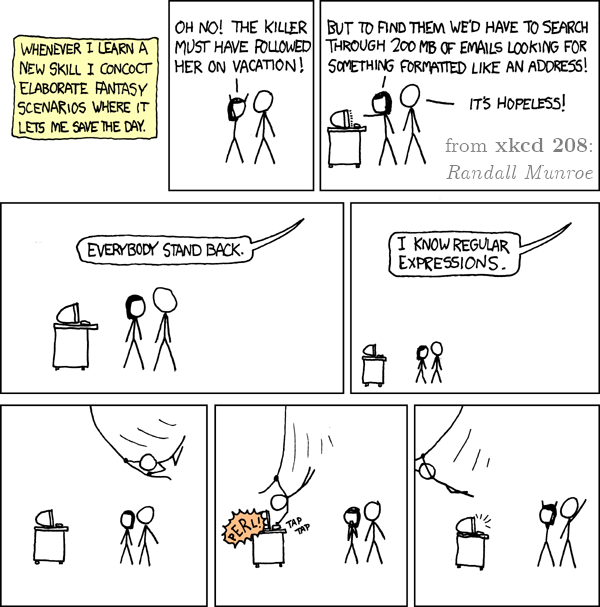
\includegraphics[height=0.85\textheight]
        {figures/regexs.png} \end{center} }
    \begin{frame}{References}
        \nocite{*}
        \bibliographystyle{alpha}
        \bibliography{slides}
    \end{frame}
    \frame{\frametitle{Acknowledgements}
        \begin{itemize}
            \item{\textbf{Concepts Lite in Practice} by \emph{R. Orr} (2016) for giving a nice and intuitive introduction to Concepts Lite TS at ACCU 2016. Some of the examples are taken from his slides and the article.}
            \item{\textbf{Generic Programming with Concepts} by \emph{A. Sutton} (2015), for presenting Concepts Lite from another angle. Many of the motivating example are based on those in his presentation too.}
            \item{I would like to thank \emph{P. Sommerlad}, for hosting the wonderful meeting in Rapperswil (2018), and allowing me to participate in the discussion on Concepts along with other topics in EWG.}
            \item{Finally, I would like to thank \emph{T. Lasser} and the other teachers and participants of ``Discovering and Teaching Modern C\texttt{++}''!}
        \end{itemize}
    }
\end{document}
